\documentclass[Kravspecifikation/Kravspec_Main.tex]{subfiles}
\begin{document}
\section{Systembeskrivelse}
I dette projekt skal der laves et "Beer pong" bord. Formålet med projekt er at tage det populære drukspil "Beer pong"; som er en kombination af ordene: "beer" og "ping pong". Og lave et bord som gør spillet: mere tilgængeligt, sjovere og mere moderne; Dette gøres ved at gøre spillet mere arkade ligende. For eksempel hvis man går ind i en arkade nu om dage, kan man normalt bare have nogle mønter/poletter med. Så kan man vælge at spille: airhockey, bordfodbold og så videre.  \newline 
Dette betyder at man ikke selv skal finde et bord, som normalt ikke er den rigtige størrelse. Man skal ikke selv have en ping pong bold med, eller finde en. Og siden det er et drukspil, så har man sandsynligvis allerede øl og kopper selv. \newline 
Systemet kommer til at bestå følgende dele: Et bord; som består af plade, ben og kop område i plade; sensorer, tre Psocs, en raspeberry Pi Zero, et display ,en bold-dispenser,betalings område, og wifi forbindelse. Forbindelse mellem disse enheder kan ses på figur \ref{fig:systemet}. \newline
Her skal bordet ses som et slags "center" for det hele, da det er der spillet kommer til at foregå: Alt det andet er bare baggrund for at styre maskineriet. Det ses også at både bordet, boldene og betalingsområdet er tilsluttet hver deres sensor del. Dette er ikke fordi der kun er en sensor, men fordi de alle bruger et antal sensorer til at registrer deres funktions områder. For eksempel registrere bordet når der løftes en kop, betalings området registrere hvornår der er betalt osv. 
De sensorer fortæller så til de psoc's der bruges hvad der sker. Ud fra det sender de information til en raspberry pi, som styre information, hjemmeside og et display som viser score, navne osv. 

\begin{figure}[H]
    \centering
    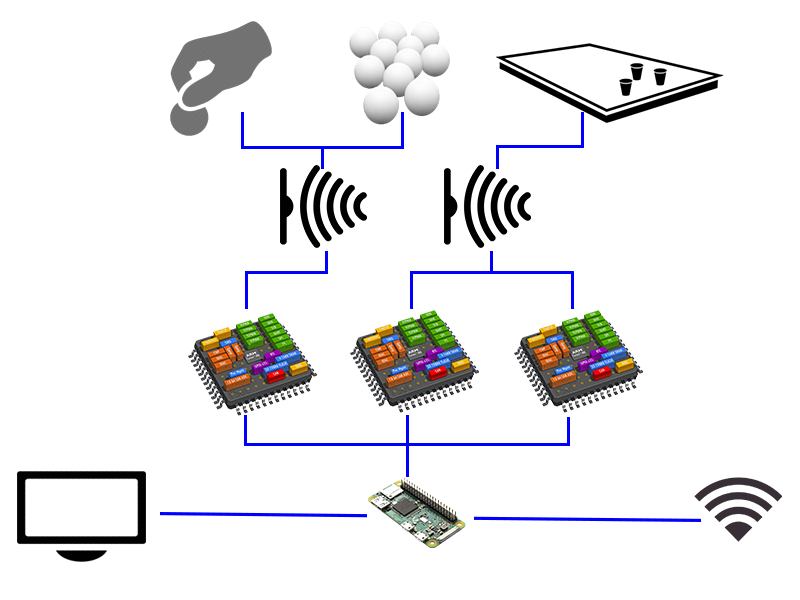
\includegraphics[scale=0.45]{Kravspecifikation/Systembeskrivelse/pics/Systembeskrivelse.png}
    \caption{Beer Pong table - Systemet}
    \label{fig:systemet}
\end{figure}


\end{document}